\chapter{Resumen del Presupuesto del Proyecto}
\label{ch:presupuesto}

En esta sección se presenta un resumen del presupuesto del proyecto, que incluye los costes de personal estimados para el desarrollo de esta primera versión del proyecto. El coste relacionado con el software y las herramientas utilizadas ha sido considerado nulo, ya que se ha hecho uso de software libre y gratuito.

Por otro lado, no se ha considerado ningún coste relacionado con la infraestructura, pues el despliegue de la aplicación se encuentra fuera del alcance del proyecto. Para hacer una estimación de sus costes se debería tener la aplicación desarrollada al completo y se debería hacer un estudio muy detallado de la arquitectura y de la infraestructura necesaria para su despliegue.

Con todo esto presente, el resumen del presupuesto del proyecto es el descrito en la tabla \ref{tab:presupuesto}.

\renewcommand{\arraystretch}{1.5}

\begin{table}[H]
    \centering
    \begin{tabular}{lc}
        \hline
        \textbf{Tipo}     & \textbf{Precio final}            \\
        \hline \hline
        \multicolumn{2}{c}{\textbf{DESARROLLO}}              \\
        \hline
        Base de datos     & 525 €                            \\
        \textit{Backend}  & 1050 €                           \\
        \textit{Frontend} & 2850 €                           \\
        \hline
        \multicolumn{2}{c}{\textbf{SOFTWARE Y HERRAMIENTAS}} \\
        \hline
        Software          & 0 €                              \\
        Herramientas      & 0 €                              \\
        \hline
        \textbf{TOTAL}    & \textbf{4425 €}                  \\
        \hline
    \end{tabular}
    \caption{Costes totales del proyecto.}
    \label{tab:presupuesto}
\end{table}

Alternativamente, se puede ver el presupuesto del proyecto en formato gráfico en la figura \ref{fig:presupuesto}.

\begin{figure}[H]
    \centering
    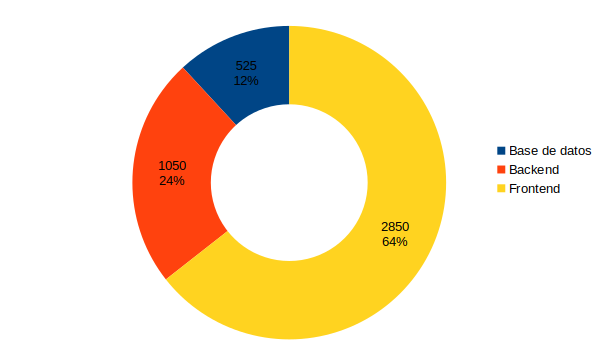
\includegraphics[width=0.8\textwidth]{figures/presupuesto/plot.png}
    \caption{Presupuesto del proyecto.}
    \label{fig:presupuesto}
\end{figure}

Por último, para una mejor comprensión de los costes del proyecto, se ha realizado un desglose detallado en el correspondiente documento de "Presupuesto", disponible en el mismo repositorio del proyecto. En este documento se pueden encontrar todos los las tareas asociadas a cada uno de los costes, así como una estimación más detallada de los tiempos invertidos en cada una de ellas. Por último, también se ha incluido en dicho documento un listado con todos los recursos de software y herramientas utilizadas.